\documentclass{article}


% if you need to pass options to natbib, use, e.g.:
%     \PassOptionsToPackage{numbers, compress}{natbib}
% before loading neurips_2024


% ready for submission
% \usepackage[final]{neurips_2024}


% to compile a preprint version, e.g., for submission to arXiv, add add the
% [preprint] option:
    \usepackage[preprint]{neurips_2024}


% to compile a camera-ready version, add the [final] option, e.g.:
%    \usepackage[final]{neurips_2024}


% to avoid loading the natbib package, add option nonatbib:
%    \usepackage[nonatbib]{neurips_2024}


\usepackage[utf8]{inputenc} % allow utf-8 input
\usepackage[T1]{fontenc}    % use 8-bit T1 fonts
\usepackage{hyperref}       % hyperlinks
\usepackage{url}            % simple URL typesetting
\usepackage{booktabs}       % professional-quality tables
\usepackage{amsfonts}       % blackboard math symbols
\usepackage{nicefrac}       % compact symbols for 1/2, etc.
\usepackage{microtype}      % microtypography
\usepackage{xcolor}         % colors
\usepackage{amsmath}
\usepackage{graphicx}
\usepackage{float}


\title{Assignment-10 \\ Linear Regression and Gradient Descent}


% The \author macro works with any number of authors. There are two commands
% used to separate the names and addresses of multiple authors: \And and \AND.
%
% Using \And between authors leaves it to LaTeX to determine where to break the
% lines. Using \AND forces a line break at that point. So, if LaTeX puts 3 of 4
% authors names on the first line, and the last on the second line, try using
% \AND instead of \And before the third author name.


\author{Harshvardhan Patidar\\
  Department of Artificial Intelligence\\
  Indian Institute of Technology Hyderabad\\
  \texttt{ai24btech11015@iith.ac.in}
  % example of co authors
  % \And
  % Coauthor \\
  % Affiliation \\
  % Address \\
}


\begin{document}\



\maketitle



%If you want to add an abstract, use below commands
%\begin{abstract}
%\end{abstract}



%use below command to get heading
%\section{Heading}

%If you don't want it to be included in the index, use
%\section*{}



%use below command to get sub-heading sort of thing
%\subsection{Style}



%use below commands for centering and url accordingly
%\begin{center}
%  \url{http://www.neurips.cc/}
%\end{center}



%Use below commmand for creating new paragraph
%\paragraph{}



%You can use below commands in the text to refer to specific sections (you need to use /label{} to where you are referring 
%\ref{gen_inst}



%use below to have nice tiny inline fractions, to increase space between them, use a tildae as in the latter
%\nicefrac{1}{4} Hello this is harshvardhan, typing his latex assignments
%\nicefrac{1}{4}~ Hello this is harshvardhan, typing his latex assignments



%for adding a footnote (vo jo page ke niche hi niche aate hai)
%\footnote{As in this example.}



%For adding a photo/figure
%\begin{figure}
%  \centering
%  \fbox{\rule[-.5cm]{0cm}{4cm} \rule[-.5cm]{4cm}{0cm}}
%  \caption{Sample figure caption.}
%\end{figure}



%For a table	
%\begin{table}
%  \caption{Sample table title}
%  \label{sample-table}
%  \centering
%  \begin{tabular}{lll}
%    \toprule
%    \multicolumn{2}{c}{Part}                   \\
%    \cmidrule(r){1-2}
%    Name     & Description     & Size ($\mu$m) \\
%    \midrule
%    Dendrite & Input terminal  & $\sim$100     \\
%    Axon     & Output terminal & $\sim$10      \\
%    Soma     & Cell body       & up to $10^6$  \\
%    \bottomrule
%  \end{tabular}
%\end{table}



%use for a giving a vertical space 
%\medskip



%Use for appendix (idk what it is)
%\appendix



%For yes, no or na
%You should answer \answerYes{}, \answerNo{}, or \answerNA{}.

\section{Linear Regression}
    \subsection{Univariate Linear Regression}
        \paragraph{}
            A univariate linear function relates the input $x$ and output $y$ in a linear relation of the form $ y = w_1x + w_0$. The coefficients are considered as weights and hence are named as w. The value of y can be altered by modifying the weights of the terms. For more general case, we will define $\textbf{w}$ to be a vector $<w_0, w_1>$ and define our function as 
            \begin{equation*}
                h_w (x) = w_1 x + w_0
            \end{equation*}
        \paragraph{}
            The process of finding the best fitting $h_w$ is called linear regression.  To find the best fit function, we will find the value of the weight $<w_0, w_1>$ which minimizes the loss function. The traditional method is to use the squared-error loss function, denoted as $L_2$, over the complete training data set.
            \begin{equation*}
                \text{Loss}(h_w) = \sum_{j=1}^{N} L_2(y_j, h_w(x_j)) = \sum_{j=1}^{N} (y_j - h_w(x_j))^2
            \end{equation*}
            where 
                \begin{equation*}
                    h_w (x) = w_1 x + w_0
                \end{equation*}
        \paragraph{}
            We will select $w^*$ such as $w^* = \arg\min_w \text{Loss}(h_w)$. The function for Loss($h_w$) can be minimized by making its partial derivative w.r.t $w_0$ and $w_1$ zero:
                \begin{equation*}
                    \frac{\partial}{\partial w_0} \sum_{j=1}^{N} (y_j - (w_1 x_j + w_0))^2 = 0 \quad \text{and} \quad
\frac{\partial}{\partial w_1} \sum_{j=1}^{N} (y_j - (w_1 x_j + w_0))^2 = 0.
                \end{equation*}
        \paragraph{}   
            These equations have a unique solution given as,
            \begin{equation*}
                w_1 = \frac{N \left( \sum x_j y_j \right) - \left( \sum x_j \right) \left( \sum y_j \right)}{N \sum x_j^2 - \left( \sum x_j \right)^2} \quad \text{and} \quad w_0 = \frac{\sum y_j - w_1 \left( \sum x_j \right)}{N}.
            \end{equation*}

        \paragraph{}
            As in this task, we are trying to find the set of weights which minimize a loss, we can plot the loss function in the 3D space, where $w_0$ and $w_1$ are the arguments. We observe that  the loss function is convex, which implies that there are no local minimas, but only global minima.

            \begin{figure}[H]
		\centering
		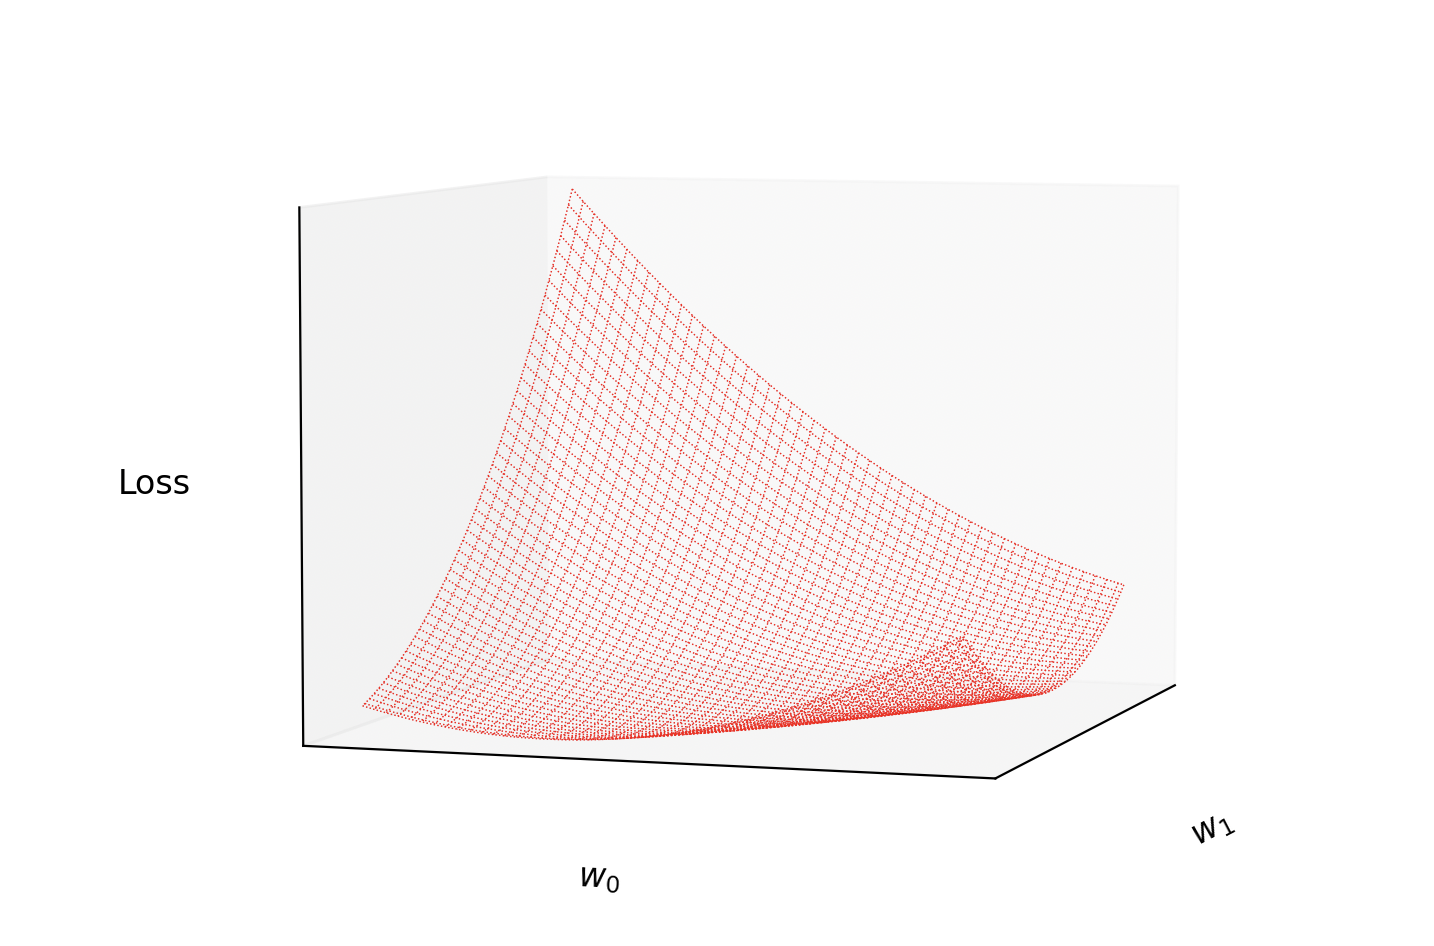
\includegraphics[width=0.5\textwidth]{plot.png}
		\caption{Plot of Loss with $w_1$ and $w_0$}
	       \end{figure}

    \subsection{Gradient Descent}
        \paragraph{}
            This method helps in minimizing the loss function without calculating the derivatives and making them zero. Instead in this method, we try for some $(w_0, w_1)$ surface, compute the approximate gradient at that point, and then move in the direction of the steepest downhill direction on the surface, to approach the minima of the loss function. Here we use a parameter $\alpha$, called the learning rate. It can be a constant or a dynamic variable depending upon the requirements.

        \paragraph{}
            Let’s first have a look at the partial derivatives of the loss function with respect to $w_1$ and $w_0$

            \begin{align*}
                \frac{\partial \text{Loss}(w)}{\partial w_i} = \frac{\partial (y - h_w(x))^2}{\partial w_i} = 2(y - h_w(x)) \times \frac{\partial (y - h_w(x))}{\partial w_i} \\
                = 2(y - h_w(x)) \times \frac{\partial (y - (w_1 x + w_0))}{\partial w_i}. \label{1}
            \end{align*}

            We get from these, 
            \begin{equation*}
                \frac{\partial \text{Loss}(w)}{\partial w_0} = -2(y - h_w(x)) \quad \text{and} \quad  \frac{\partial \text{Loss}(w)}{\partial w_1} = -2(y - h_w(x)) \times x
            \end{equation*}`
            So, after for every point $(w_0, w_1)$, we will update them as below for all the training examples
                \begin{equation*}
                    w_0 \leftarrow w_0 + \alpha \sum (y_j - h_w(x_j))
 \quad \text{and} \quad w_1 \leftarrow w_1 + \alpha \sum (y_j - h_w(x_j)) \times x_j
                \end{equation*}

        \paragraph{}
            These updates constitute the batch gradient descent learning rule. We call one step, that covers the complete training examples as an epoch. This method is slow as we need to sum the partial derivatives over all the training examples, which might be computationally expensive. To consider this, we use another method called Stochastic Gradient Descent (SGD).
        \paragraph{}
            The SGD selects only a few training examples to update the values of the wrights at each step rather than considering the complete training set. If we take $N/\eta$ examples for consideration, our calculations reduce by a factor of $\eta$, and our error increases only by a factor of $\sqrt{\eta}$. The $\eta$ can be considered as an hyperparameter which needs to be specifically tuned for ever problem.
        \paragraph{}
            SGD is laso effective when enw data is coming one-by-one, in the absence of the stationarity assumption. (SGD is also known as Online GradIent descent). SGD works significantly nice in cases where there are multiple local minimas as well.
            \newpage
    \subsection{Multivariable Linear Regression}
        `\paragraph{}
            We can consider multivariable linear regressions as well, where our input $\mathbf{x}_j$ is an $n$-element vector. Here,
            \begin{equation*}
                h_w(x_j) = w_0 + w_1 x_{j,1} + \cdots + w_n x_{j,n} = w_0 + \sum_{i=1}^{n} w_i x_{j,i}
            \end{equation*}
            We can make it beautiful by adding the lingering $w_0$ in the $\mathbf{w}$ and introducing a new attribute $x_{j,0}$ which has value as 1. Then $h$ is simply the dot product of weights and the input vector.
            \begin{equation*}
                h_{\mathbf{w}}(\mathbf{x}_j) = \mathbf{w} \cdot \mathbf{x}_j = \mathbf{w}^{\top} \mathbf{x}_j = \sum_{i=1}^{n} w_i x_{j,i}
            \end{equation*}

            We then select the best vector $w^*$ which minimizes the loss function
            \begin{equation*}
                \mathbf{w}^* = \arg\min \sum L_2(y_j, \mathbf{w} \cdot \mathbf{x}_j)
            \end{equation*}

            For updating the weights, we can still use the same previous formula, with slight modifications
            \begin{equation*}
                w_i \leftarrow w_i + \alpha \sum (y_j - h_{\mathbf{w}}(\mathbf{x}_j)) \times x_{j,i}
            \end{equation*}

            The feasible \textbf{w} can also be found analytically by using linear algebra and vector calculus. The predicted output vector is $\hat{\mathbf{y}} = \mathbf{Xw}$, then the squared loss error is 
            \begin{equation*}
                \mathbf{L}(\mathbf{w}) = \| \hat{\mathbf{y}} - \mathbf{y} \|_2 = \| \mathbf{X} \mathbf{w} - \mathbf{y} \|_2
            \end{equation*}

                To minimize, we make the gradient zero,
                \begin{align*}
                    \nabla_{\mathbf{w}} L(\mathbf{w}) = 2 \mathbf{X}^{\top} (\mathbf{X} \mathbf{w} - \mathbf{y}) = 0\\
                    \Rightarrow \mathbf{w}^* = (\mathbf{X}^{\top} \mathbf{X})^{-1} \mathbf{X}^{\top} \mathbf{y}
                \end{align*}

                The expression $(\mathbf{X}^{\top} \mathbf{X})^{-1} \mathbf{X}^{\top} $ is called the pseudoinverse of the data matrix, and the above equation is called as the normal equation.

\newpage
\section{The Gradient Method}
    \paragraph{}
        This paper was authored by Louis Augustin Cauchy in 1847. In this paper Cauchy tried to solve the algebraic equations which represented the heavenly bodies and their movements. His motivation was the complex differential equations which required to be solved to get a solution for such problems, which he didn’t want to do. So he tried to find the solutions directly, instead of finding the differential equations and thus giving this beautiful method, called the Gradient Method.
    \paragraph{}
        His aim was to find those values of the variables $x,y,z, \ldots$ which minimized the function $u$, taking variables $x,y,z, \dots$ as input, is always non-negative and is continuous.
    \begin{equation*}
        u=f(x,y,z,\ldots)
    \end{equation*}

        He tried to indefinitely decrease the function $u$ to its minimum value, by altering the variables, to continuously decrease the value of $u$. For this, he calculated the derivatives 
    \begin{equation*}
        X = f'_{x}, \quad Y = f'_{y}, \quad Z = f'_{z}, \ldots
    \end{equation*}

        And gave small increment/decrement $\alpha, \beta, \gamma, \ldots$ respectively to $x,y,z, \ldots$
    \begin{equation*}
        f(x + \alpha, y + \beta, z + \gamma, \ldots) = u + X\alpha + Y\beta + Z\gamma + \ldots
    \end{equation*}

        He replaced the $\alpha, \beta, \gamma, \ldots$ as below by introducing a decrement parameter $\theta$:
        \begin{equation*}
            \alpha = -\theta X, \quad \beta = -\theta Y, \quad \gamma = -\theta Z, \ldots 
        \end{equation*}

        Then $u$ was calculated approximately as
        \begin{equation*}
            f(x - \theta X, y - \theta Y, z - \theta Z, \ldots) = u - \theta (X^2 + Y^2 + Z^2 + \ldots)
        \end{equation*}

        This way as $\theta$ varies, $u$ also decreases and eventually obtains its minimum value.

    \paragraph{}
        He mentioned Convergence as, that if the new value of $u$ is not the smallest, an even smaller value can be found by proceeding in a similar manner. He was not fully confident that this might not always find the solution as this was an approximation only and not complete calculation. 
        On the contrary, he was convinced that $u$ will always converge to its minimum value. This was a significant contribution by one of the notable mathematicians of that time which is still used. 


            

            

   



\end{document}
